\documentclass[tikz,border=4pt]{standalone}
\usepackage[T1]{fontenc}
\usepackage{lmodern}
\usetikzlibrary{arrows.meta,positioning,fit,backgrounds,calc}
\begin{document}
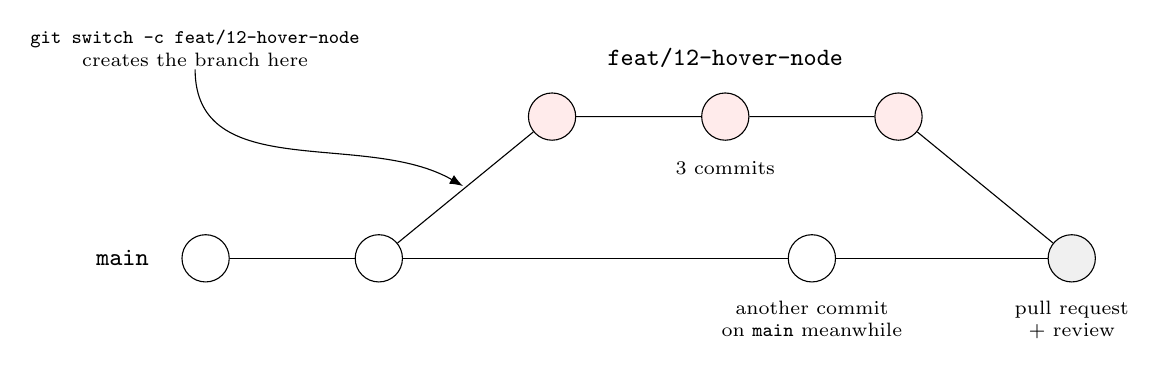
\begin{tikzpicture}[
  cmt/.style={draw,circle,minimum size=6mm,inner sep=0pt,fill=white},
  mine/.style={cmt,fill=red!8},
  mrg/.style={cmt,fill=gray!12},
  lab/.style={font=\scriptsize,fill=white,inner sep=1pt,align=center},
  >={Latex}]
\node[cmt] (m0) at (0,0) {};
\node[cmt] (m1) at (2.2,0) {};
\node[cmt] (m2) at (7.7,0) {};
\node[mrg] (mm) at (11,0) {};
\node[mine] (b1) at (4.4,1.8) {};
\node[mine] (b2) at (6.6,1.8) {};
\node[mine] (b3) at (8.8,1.8) {};
\draw (m0) -- (m1) -- (m2) -- (mm);
\draw (m1) -- (b1) -- (b2) -- (b3) -- (mm);
\node[font=\small,anchor=east] at (-0.6,0) {\texttt{main}};
\node[font=\small,anchor=south] at (6.6,2.3) {\texttt{feat/12-hover-node}};
\node[lab,anchor=north] at (7.7,-0.5) {another commit\\on \texttt{main} meanwhile};
\node[lab,anchor=north] at (11,-0.5) {pull request\\+ review};
\node[lab,anchor=south east] (sw) at (2.0,2.4) {\texttt{git switch -c feat/12-hover-node}\\creates the branch here};
\draw[->,shorten >=1pt] (sw.south) to[out=-90,in=150] ($(m1)!0.5!(b1)$);
\node[lab] at (6.6,1.15) {3 commits};
\end{tikzpicture}
\end{document}
